\vspace*{4mm}
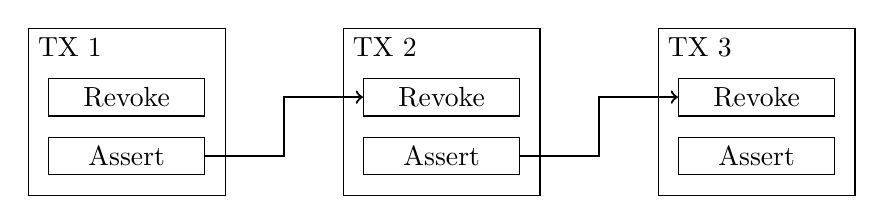
\begin{tikzpicture}
% \node at (-1, 2.5) {Inputs};
% \node at (5, 2.5) {Outputs};
\draw (0, 0.75) rectangle (2.5,2.875);
\node[below right] at (0, 2.875) {TX 1};
\node[draw, text width=1.75cm, align=center] (Revoke 1) at (1.25,2) {Revoke};
\node[draw, text width=1.75cm, align=center] (Assert 1) at (1.25,1.25) {Assert};

\draw (4, 0.75) rectangle (6.5,2.875);
\node[below right] at (4, 2.875) {TX 2};
\node[draw, text width=1.75cm, align=center] (Revoke 2) at (5.25,2) {Revoke};
\node[draw, text width=1.75cm, align=center] (Assert 2) at (5.25,1.25) {Assert};

\draw (8, 0.75) rectangle (10.5,2.875);
\node[below right] at (8, 2.875) {TX 3};
\node[draw, text width=1.75cm, align=center] (Revoke 3) at (9.25,2) {Revoke};
\node[draw, text width=1.75cm, align=center] (Assert 3) at (9.25,1.25) {Assert};

\draw[->, thick] (Assert 1) -| (3.25, 2) |- (Revoke 2);
\draw[->, thick] (Assert 2) -| (7.25, 2) |- (Revoke 3);
\end{tikzpicture}
\vspace*{4mm}
